
\documentclass{../concepts/titul_zprava_p/prepareprotokolZprava} %všechny balíčky pro protokol + titulní strana

\usepackage{graphicx}
\usepackage{newfloat}
\usepackage{caption}
\usepackage{booktabs}
\usepackage{amssymb}
\usepackage{amsmath}
\usepackage{siunitx}
\usepackage{textcomp}
\usepackage{comment}
\usepackage{gensymb}
\usepackage{subcaption}
\usepackage{multirow}
\sisetup{inter-unit-product =$\cdot$}
%\sisetup{separate-uncertainty=true}

\praktikum{III} %číslo praktika (I, II nebo III)
\autor{David Němec} %jméno autora
\datum{7.\,4.\,2026} %datum měření
\cislo{2} %číslo úlohy
\nazev{Měření parametrů zobrazovacích soustav} %název úlohy

\DeclareFloatingEnvironment[fileext=los, placement={htbp}, name=Obrázek]{schema}

\newcommand{\nobars}{
Chybové úsečky nebyly pro~svou malou velikost pro~přehlednost vykresleny.}

\newcommand{\nohbars}{
Horizontální chybové úsečky nebyly pro~svou malou velikost pro~přehlednost vykresleny.}

\newcommand{\novbars}{
Vertikální chybové úsečky nebyly pro~svou malou velikost pro~přehlednost vykresleny.}

\newcommand{\relative}[1]{
\frac{\sigma_{#1}}{#1}
}
\newcommand{\squared}[1]{
\left( #1 \right)^2
}
\newcommand{\relsqr}[1]{
\squared{\relative{#1}}
%\left( \frac{\sigma_{#1}}{#1} \right)^2
}

\begin{document}
\renewcommand{\figurename}{Graf}
\renewcommand{\refname}{Literatura}
\renewcommand{\today}{\number\day.\,\number\month.\,\number\year}

% add another graphics path to find ZPF.pdf for title page
% now searches for images in ./ and ../concepts/titul_protokol_p/
\graphicspath{{../concepts/titul_protokol_p/}}
\maketitle

% ========================== PRACOVNÍ ÚKOL ============================
\section{Pracovní úkoly}
\begin{enumerate}
    \item Změřte ohniskovou vzdálenost tenké ploskovypuklé čočky jednak Besselovou metodou, jednak metodou dvojího zvětšení.
    \item Změřte kulovou vadu tenké ploskovypuklé čočky měřené v bodě 1. v~obou směrech a~pro~dvě vzdálenosti předmětu 
    $a = \qty{30}{cm}$, $a = \qty{60}{cm}$. Získané výsledky těchto čtyř uspořádání zpracujte do~jednoho grafu a~diskutujte 
    velikost kulové vady v jednotlivých případech.
    \item Na fokometru změřte optickou mohutnost čočky měřené v bodě 1. a výsledek srovnejte s výsledky měření ohniskové vzdálenosti.
    \item Užitím goniometru určete vzdálenost hlavních rovin čočky měřené v bodě 1. a tlusté ploskovypuklé čočky.
    \item S použitím změřené vzdálenosti hlavních rovin vypočítejte systematickou chybu, které se dopouštíme při~měření ohniskové 
    vzdálenosti Besselovou metodou. Diskutujte, která z uvedených metod měření ohniskové vzdálenosti je v uvedeném uspořádání 
    přesnější. Porovnejte relativní chyby měření.
    \item Ze změřené tloušťky tlusté ploskovypuklé čočky a změřené vzdálenosti hlavních rovin určete index lomu skla.
\end{enumerate}

% ============================= TEORIE ================================

% ======================== rovnice a definiční vztahy ------- asi hotovo
\section{Vztahy a veličiny}

Ohnisková vzdálenost tenké čočky určená Besselovou metodou se vypočítá podle vztahu \cite{studijni}
\begin{equation}
    \label{eq:bessel}
    f = \frac{D^2 - \Delta^2}{4 D} \,,
\end{equation}
kde $D$ je vzdálenost mezi předmětem a~obrazem a~$\Delta$ je vzdálenost mezi dvěma polohami čočky, pro~které na~stínítku vznikne
ostrý obraz. Pro~tlustou čočku s~nenulovou vzdáleností hlavních rovin $\delta$ platí upravený vztah \cite{studijni}
\begin{equation}
    \label{eq:bessel_tlusta}
    f = \frac{\left(D-\delta\right)^2 - \Delta^2}{4 \left(D - \delta\right)}\,.
\end{equation}

Ohnisková vzdálenost čočky určená metodou dvojího zvětšení se vypočítá podle vztahu \cite{studijni}
\begin{equation}
    \label{eq:dvoji_zvetseni}
    f = \frac{\left| a_1' - a_2' \right|}{\left| \left(\frac{Y'}{Y}\right)_2 - \left(\frac{Y'}{Y}\right)_1 \right|} = 
    \frac{\Delta}{\left| \left(\frac{Y'}{Y}\right)_2 - \left(\frac{Y'}{Y}\right)_1 \right|}\,,
\end{equation}
kde $a_1'$ a~$a_2'$ jsou vzdálenosti obrazu od čočky v~polohách 1 a~2, jejich rozdíl je tedy roven $\Delta$, $Y'$ je 
velikost obrazu a~$Y$ je velikost předmětu,
indexy 1 a~2 u~příčných zvětšení (poměrů $\frac{Y'}{Y}$) odpovídají polohám 1 a~2.

Sférická (kulová) vada čočky je definována vztahem \cite{studijni}
\begin{equation}
    \label{eq:kulova_vada_definice}
    \Delta a' = a' - a_p' \,,
\end{equation}
kde $a'$ je vzdálenost obrazu od čočky pro~paprsky procházející čočkou ve~vzdálenosti $s$ od~optické osy čočky a~$a_p'$
je vzdálenost obrazu od~čočky pro~paraxiální paprsky.
Pro~soustavu tvořenou jednou čočkou platí přibližný vztah \cite{studijni}
\begin{equation}
    \label{eq:kulova_vada_na_s}
    \Delta a' \approx K s^2 \,,
\end{equation}
kde $K$ je konstanta. Pro~spojku platí $K < 0$.

Střední poloměr $s$ clony s~výřezem ve~tvaru mezikruží se~vypočítá podle vztahu (upraveno podle \cite{studijni}):
\begin{equation}
    \label{eq:stredni_polomer_mezikruzi}
    s = \frac{d_1 + d_2}{4} \,,
\end{equation}
kde $d_1$ a~$d_2$ jsou vnitřní a~vnější průměr mezikruží.

Optická mohutnost čočky je definována jako \cite{wiki}
\begin{equation}
    \label{eq:mohutnost}
    \varphi = \frac{1}{f} \,,
\end{equation}
kde $f$ je ohnisková vzdálenost čočky.

Index lomu skla tlusté plankonvexní čočky lze vypočítat podle vztahu (upraveno podle \cite{studijni})
\begin{equation}
    \label{eq:index_lomu}
    n = \frac{t}{t-\delta} \,,
\end{equation}
kde $t$ je tloušťka čočky a~$\delta$ je vzdálenost hlavních rovin čočky. Vzdálenost hlavních rovin
se~určí pomocí goniometru umožňujícího posuv čočky jako rozdíl takových poloh, pro~které osa otáčení goniometru
prochází jedním a~druhým hlavním bodem čočky. Ty jsou totožné s~uzlovými body čočky, ve kterých jsou paprsky dopadající 
na~čočku rovnoběžné s~vystupujícími paprsky.


% ============= schémata asi nejsou nutná
% \begin{schema}[!htbp]
%     \centering
%     %\includegraphics[width=0.5\linewidth]{image.png}
%     \caption{Schéma PŘÍSTROJE \cite{pokyny}}
%     \label{sch:pristroj}
% \end{schema}


% ======================== VÝSLEDKY MĚŘENÍ ===========================
\section{Výsledky a zpracování měření}

% ============= podmínky měření ------------ asi hotovo
% zde nejsou důležité

% ============= přístroje a jejich nejistoty ----------asi hotovo
\subsection{Použité měřicí přístroje}
\begin{enumerate}
    \item Pásové měřidlo - použité pro~měření vzdáleností předmětu, obrazu a~čočky, nejistota $\sigma_{x,B} = \qty{1}{mm}$.
    \item Matnice se~stupnicí - použitá pro~měření velikosti obrazu, nejistota $\sigma_{y',B} = \qty{0.1}{mm}$.
    \item Posuvné měřítko - použité pro~měření vnitřních a~vnějších poloměrů clon s~výřezy ve~tvaru mezikruží,
    nejistota $\sigma_{d,B} = \qty{0.1}{mm}$.
    \item Digitální posuvné měřítko - použité pro~měření tloušťky čočky, nejistota $\sigma_{t,B} = \qty{0.01}{mm}$.
    \item Posuvná stupnice goniometru - použitá pro~určení pozic hlavních rovin čočky, nejistota $\sigma_{h,B} = \qty{0.1}{mm}$.
    \item Fokometr F-910 - použitý pro~měření optické mohutnosti čočky, nejistota $\sigma_\varphi = \qty{0.25}{D}$.
\end{enumerate}

% ============= naměřené hodnoty, vypočtené veličiny, grafy, výsledky
\subsection{Naměřené hodnoty a výpočty}

Měření probíhalo se~sodíkovou výbojkou o~vlnové délce $\lambda_\mathrm{Na} = \qty{589.3}{nm}$ \cite{vlnovedelky}.

% ================== ohniskove vzdalenosti ----------- asi hotovo
\subsubsection{Ohniskové vzdálenosti Besselovou metodou a metodou dvojího zvětšení}

Nejistota průměrné hodnoty pozice čočky $x$ a~pozice okrajů obrazu $y_l'$ a~$y_r'$ byla určena podle \cite{englich} jako 
nejistota aritmetického průměru patřičně zvětšená o~nejistotu měřidla (nejistota jedné naměřené hodnoty je daná
rozptylem hodnot a~nejistotou měřidla)
\begin{equation}
    \label{eq:sigma_mean_x_yl_yr}
    \sigma_{\overline{\theta}} = \sqrt{ \frac{1}{4 \cdot 5} \sum_{i=1}^{5} \left( \theta_i - \overline{\theta} \right)^2 +
    \frac{1}{5} \sigma_{\theta,B}^2 } \; \mathrm{, kde } \; \theta = x, y_l', y_r' \;\mathrm{ a }\; 
    \sigma_{y_l',B}=\sigma_{y_r',B} = \sigma_{y',B} = \qty{0.01}{cm}\,.
\end{equation}

\begin{table}[!htbp]
\centering
\caption{Opakované měření pozic čočky a~okrajů obrazu pro~obě polohy čočky a~pro~čtyři různé vzdálenosti předmětu a~obrazu $D$.}
\begin{tabular}{c|ccc|ccc}
 \toprule
  & \multicolumn{3}{c|}{poloha 1} & \multicolumn{3}{c}{poloha 2} \\
 \midrule
  & $x\, (\mathrm{cm})$ & $y_l'\, (\mathrm{cm})$ & $y_r'\, (\mathrm{cm})$ & $x\, (\mathrm{cm})$ & $y_l'\, (\mathrm{cm})$ & $y_r'\, (\mathrm{cm})$ \\
 \midrule
 \multirow{5}{*}{$D=\qty{84}{cm}$} & $40.1(1)$ & $10.81(1)$ & $12.34(1)$ & $56.8(1)$ & $11.33(1)$ & $12.00(1)$ \\
  & $40.1(1)$ & $10.80(1)$ & $12.30(1)$ & $56.8(1)$ & $11.33(1)$ & $11.99(1)$ \\
  & $39.6(1)$ & $10.81(1)$ & $12.31(1)$ & $56.6(1)$ & $11.32(1)$ & $11.98(1)$ \\
  & $39.7(1)$ & $10.81(1)$ & $12.32(1)$ & $56.9(1)$ & $11.32(1)$ & $11.98(1)$ \\
  & $40.0(1)$ & $10.80(1)$ & $12.32(1)$ & $56.6(1)$ & $11.32(1)$ & $11.99(1)$ \\
  \midrule
  průměr & $39.90(14)$ & $10.806(2)$ & $12.318(7)$ & $56.74(12)$ & $11.324(2)$ & $11.988(4)$ \\
  \midrule
  \midrule
  \multirow{5}{*}{$D=\qty{94}{cm}$}& $35.6(1)$ & $10.38(1)$ & $12.59(1)$ & $71.0(1)$ & $9.46(1)$ & $9.92(1)$ \\
  & $35.4(1)$ & $10.37(1)$ & $12.58(1)$ & $70.7(1)$ & $9.47(1)$ & $9.93(1)$ \\
  & $35.7(1)$ & $10.37(1)$ & $12.58(1)$ & $70.8(1)$ & $9.47(1)$ & $9.92(1)$ \\
  & $35.5(1)$ & $10.37(1)$ & $12.59(1)$ & $70.9(1)$ & $9.48(1)$ & $9.92(1)$ \\
  & $35.6(1)$ & $10.37(1)$ & $12.59(1)$ & $70.9(1)$ & $9.48(1)$ & $9.92(1)$ \\
  \midrule
  průměr & $35.56(11)$ & $10.372(2)$ & $12.586(2)$ & $70.86(11)$ & $9.472(4)$ & $9.922(2)$ \\
  \midrule
  \midrule
  \multirow{5}{*}{$D=\qty{104}{cm}$} & $33.8(1)$ & $8.00(1)$ & $10.81(1)$ & $82.7(1)$ & $9.52(1)$ & $9.86(1)$ \\
  & $33.7(1)$ & $8.01(1)$ & $10.80(1)$ & $83.2(1)$ & $9.52(1)$ & $9.87(1)$ \\
  & $33.7(1)$ & $8.00(1)$ & $10.80(1)$ & $83.0(1)$ & $9.53(1)$ & $9.87(1)$ \\
  & $34.0(1)$ & $8.01(1)$ & $10.80(1)$ & $82.9(1)$ & $9.52(1)$ & $9.87(1)$ \\
  & $33.9(1)$ & $8.00(1)$ & $10.80(1)$ & $83.1(1)$ & $9.52(1)$ & $9.88(1)$ \\
  \midrule
  průměr & $33.82(12)$ & $8.004(2)$ & $10.802(2)$ & $82.98(13)$ & $9.522(2)$ & $9.870(3)$ \\
    \midrule
    \midrule
  \multirow{5}{*}{$D=\qty{89}{cm}$}& $37.1(1)$ & $8.60(1)$ & $10.50(1)$ & $64.2(1)$ & $9.46(1)$ & $9.98(1)$ \\
  & $37.4(1)$ & $8.60(1)$ & $10.51(1)$ & $64.5(1)$ & $9.45(1)$ & $9.98(1)$ \\
  & $37.1(1)$ & $8.60(1)$ & $10.50(1)$ & $64.4(1)$ & $9.46(1)$ & $9.98(1)$ \\
  & $37.2(1)$ & $8.60(1)$ & $10.50(1)$ & $64.4(1)$ & $9.46(1)$ & $9.98(1)$ \\
  & $37.5(1)$ & $8.59(1)$ & $10.50(1)$ & $64.3(1)$ & $9.47(1)$ & $9.97(1)$ \\
  \midrule
  průměr & $37.26(13)$ & $8.598(2)$ & $10.502(2)$ & $64.36(11)$ & $9.460(3)$ & $9.978(2)$ \\
 \bottomrule
\end{tabular}
\label{tab:raw_data}
\end{table}

Vzdálenost pozic čočky mezi polohami 1 a~2 byla určena jako $\Delta = x_2 - x_1$ a~její nejistota podle \cite{englich} jako:
\begin{equation}
    \label{eq:sigma_delta}
    \sigma_{\Delta} = \sqrt{\sigma_{x_2}^2 + \sigma_{x_1}^2} \,.
\end{equation}

Velikost obrazu $Y'$ se určí jako $Y' = y_r' - y_l'$ a~její nejistota podle \cite{englich} jako:
\begin{equation}
    \label{eq:sigma_Y}
    \sigma_{Y'} = \sqrt{2} \sigma_{r,B} \doteq \qty{0.014}{cm} \,.
\end{equation}

Nejistota příčného zvětšení $\frac{Y'}{Y}$ se určí podle \cite{englich} jako:
\begin{equation}
    \label{eq:sigma_YkuY}
    \sigma_{\frac{Y'}{Y}} = \frac{Y'}{Y} \sqrt{\relsqr{Y'} + \relsqr{Y}} \,,
\end{equation}
kde $\sigma_Y = \sigma_{r,B} = \qty{0.01}{cm}$ je nejistota velikosti předmětu. Předmětem byl kruhový výřez clony 
o~průměru $Y = \qty{1.00(1)}{cm}$.


\begin{table}[!htbp]
\centering
\caption{Polohy čočky, velikosti obrazů a~příčná zvětšení pro~obě polohy čočky a~pro~čtyři různé vzdálenosti předmětu a~obrazu $D$}
\begin{tabular}{c|ccc|ccc|c}
 \toprule
 & \multicolumn{3}{c|}{poloha 1} & \multicolumn{3}{c|}{poloha 2} & vzdálenost pozic čočky \\
 \midrule
 $D\, (\mathrm{cm})$ & $x\, (\mathrm{cm})$ & $Y'\, (\mathrm{cm})$ & $\frac{Y'}{{Y}}$ & $x\, (\mathrm{cm})$ & $Y'\, (\mathrm{cm})$ & $\frac{Y'}{{Y}}$ & $\Delta\, (\mathrm{cm})$ \\
 \midrule
 $84.0(1)$ & $39.90(14)$ & $1.512(7)$ & $1.512(17)$ & $56.74(12)$ & $0.664(5)$ & $0.664(8)$ & $16.84(19)$ \\
 $94.0(1)$ & $35.56(11)$ & $2.214(3)$ & $2.21(2)$ & $70.86(11)$ & $0.450(4)$ & $0.450(6)$ & $35.30(16)$ \\
 $104.0(1)$ & $33.82(12)$ & $2.798(3)$ & $2.80(3)$ & $82.98(13)$ & $0.348(4)$ & $0.348(5)$ & $49.16(18)$ \\
 $89.0(1)$ & $37.26(13)$ & $1.904(3)$ & $1.90(2)$ & $64.36(11)$ & $0.518(4)$ & $0.518(6)$ & $27.10(17)$ \\
 \bottomrule
\end{tabular}
\label{tab:prumer_data}
\end{table}

Ohnisková vzdálenost určená Besselovou metodou byla vypočtena podle vztahu \ref{eq:bessel} a~její nejistota podle \cite{englich} jako:
\begin{equation}
    \label{eq:sigma_f_bessel}
    \sigma_{f_{Bessel}} = \sqrt{ \left(\frac{D^2 + \Delta^2}{4 D^2}\right)^2 \sigma_D^2 + 
    \left(\frac{\Delta}{2 D}\right)^2 \sigma_{\Delta}^2 } \,.
\end{equation}

Ohnisková vzdálenost určená metodou dvojího zvětšení byla vypočtena podle vztahu \ref{eq:dvoji_zvetseni} a~její nejistota podle \cite{englich} jako:
% (ve všech čtyřech případech vyšlo $\left(\frac{Y'}{Y}\right)_2 < \left(\frac{Y'}{Y}\right)_1$, absolutní hodnota prohodí
% znaménko):
\begin{equation}
    \label{eq:sigma_f_dvoji}
    \sigma_{f_{dvoji}} = f_{dvoji} \sqrt{ \relsqr{\Delta} + \relsqr{\left(\frac{Y'}{Y}\right)_2} 
    + \relsqr{\left(\frac{Y'}{Y}\right)_1} } \,.
\end{equation}

Nejistoty průměrných hodnot ohniskové vzdálenosti byly vypočteny jako nejistota aritmetického průměru (daná rozptylem
hodnot) zvětšená o~nejistoty jednotlivých měření:
\begin{equation}
    \label{eq:sigma_mean_f}
    \sigma_{\overline{f}} = \sqrt{ \frac{1}{3 \cdot 4} \sum_{i=1}^{4} \left( f_i - \overline{f} \right)^2
    + \frac{1}{16} \sum_{i=1}^{4} \sigma_{f_i}^2 } \,.
\end{equation}

\begin{table}[!htbp]
\centering
\caption{Vypočtené ohniskové vzdálenosti Besselovou metodou a~metodou dvojího zvětšení pro~čtyři různé vzdálenosti předmětu
a~obrazu $D$.}
\begin{tabular}{ccc}
 \toprule
 $D\, (\mathrm{cm})$ & $f_{Bessel}\, (\mathrm{cm})$ & $f_{dvoji}\, (\mathrm{cm})$ \\
 \midrule
 $84.0(1)$ & $20.16(6)$ & $19.9(5)$ \\
 $94.0(1)$ & $20.19(6)$ & $20.0(3)$ \\
 $104.0(1)$ & $20.19(7)$ & $20.1(2)$ \\
 $89.0(1)$ & $20.19(6)$ & $19.6(3)$ \\
 \midrule
 průměr & $20.18(3)$ & $19.9(2)$ \\
 \bottomrule
\end{tabular}
\label{tab:ohniskove_vzdalenosti}
\end{table}

% ================== fokometr ------------- asi hotovo
\subsubsection{Ohnisková vzdálenost z Fokometru}
Z~optické mohutnosti čočky $\varphi = \qty{5.3(3)}{D}$ odečtené z~fokometru byla vypočtena ohnisková vzdálenost 
podle vztahu (\ref{eq:mohutnost}) jako $f_{fokometr} = \qty{19.0(9)}{cm}$
přičemž~její nejistota je daná vztahem \cite{englich}:
\begin{equation}
    \label{eq:sigma_f_mohutnost}
    \sigma_{f_{fokometr}} = f_{fokometr} \relative{\varphi} \,.
\end{equation}


% ===================== kulova vada ----------------- asi hotovo
\subsubsection{Kulová vada}

Nejistota středního poloměru výřezu clony ve~tvaru mezikruží byla určena jako
\begin{equation}
    \label{eq:sigma_s}
    \sigma_s = \frac{\sqrt{2}}{4} \sigma_{d,B} \doteq \qty{0.004}{cm} \,.
\end{equation}

\begin{table}[!htbp]
\centering
\caption{Vnější a~vnitřní průměry výřezů clon a~jejich střední poloměry. Výřez clony $0$ je jen kruhový otvor.}
\begin{tabular}{cccc}
 \toprule
 clona & $d_2\, (\mathrm{cm})$ & $d_1\, (\mathrm{cm})$ & $s\, (\mathrm{cm})$ \\
 \midrule
 $0$ & $1.00(1)$ & $0.00(0)$ & $0.250(4)$ \\
 $1$ & $2.00(1)$ & $1.00(1)$ & $0.750(4)$ \\
 $2$ & $3.00(1)$ & $2.00(1)$ & $1.250(4)$ \\
 $3$ & $4.00(1)$ & $3.00(1)$ & $1.750(4)$ \\
 $4$ & $5.00(1)$ & $4.00(1)$ & $2.250(4)$ \\
 \bottomrule
\end{tabular}
\label{tab:clony}
\end{table}

Nejistota kulové vady (spočtené jako rozdíl vzdáleností obrazu od čočky pro~paprsky procházející clonou $i\in \{1,2,3,4\}$ 
a~clonou $0$) byla vypočtena podle vztahu
\begin{equation}
    \label{eq:sigma_delta_a}
    \sigma_{\Delta a'} = \sqrt{2} \sigma_{x'} \doteq \qty{0.3}{cm} \,,
\end{equation} 
kde $\sigma_{x'} = \qty{0.2}{cm}$ (nejistota vzdálenosti obrazu od čočky) byla odhadnuta jako nejistota jednoho měření
při~určování ohniskové vzdálenosti Besselovou metodou a~metodou dvojího zvětšení.

\begin{table}[!htbp]
\centering
\caption{Vzdálenosti obrazu od čočky a příslušné kulové vady pro paprsky procházející ve~vzdálenosti $s$ od~optické osy
pro~vzdálenosti čočky a~předmětu $30$ a~$\qty{60}{cm}$ a~pro oba směry průchodu paprsků čočkou (označení je podle strany,
kterou paprsky do~čočky vstupují.)}
\begin{tabular}{cc|cc|cc|cc|cc}
 \toprule
 & & \multicolumn{2}{c|}{vypuklá \qty{30}{cm}} & \multicolumn{2}{c|}{vypuklá \qty{60}{cm}} & \multicolumn{2}{c|}{plochá \qty{30}{cm}}
 & \multicolumn{2}{c}{plochá \qty{60}{cm}} \\
 \midrule
 clona & $s\,(\unit{cm})$ & $a'\, (\mathrm{cm})$ & $\Delta a'\, (\mathrm{cm})$ & $a'\, (\mathrm{cm})$ & $\Delta a'\, (\mathrm{cm})$ & $a'\, (\mathrm{cm})$ & $\Delta a'\, (\mathrm{cm})$ & $a'\, (\mathrm{cm})$ & $\Delta a'\, (\mathrm{cm})$ \\
 \midrule
 $0$ & $0.250(4)$ & $63.5(1)$ & $0.00(14)$ & $30.5(1)$ & $0.00(14)$ & $61.0(1)$ & $0.00(14)$ & $31.0(1)$ & $0.00(14)$ \\
 $1$ & $0.750(4)$ & $63.5(1)$ & $0.00(14)$ & $30.4(1)$ & $-0.10(14)$ & $60.9(1)$ & $-0.10(14)$ & $31.0(1)$ & $0.00(14)$ \\
 $2$ & $1.250(4)$ & $62.5(1)$ & $-1.00(14)$ & $30.3(1)$ & $-0.20(14)$ & $60.4(1)$ & $-0.60(14)$ & $30.8(1)$ & $-0.20(14)$ \\
 $3$ & $1.750(4)$ & $61.0(1)$ & $-2.50(14)$ & $30.3(1)$ & $-0.20(14)$ & $60.0(1)$ & $-1.00(14)$ & $30.4(1)$ & $-0.60(14)$ \\
 $4$ & $2.250(4)$ & $59.0(1)$ & $-4.50(14)$ & $30.1(1)$ & $-0.40(14)$ & $58.5(1)$ & $-2.50(14)$ & $29.6(1)$ & $-1.40(14)$ \\
 \bottomrule
\end{tabular}
\label{tab:kulova_vada}
\end{table}

\begin{figure}
    \centering
    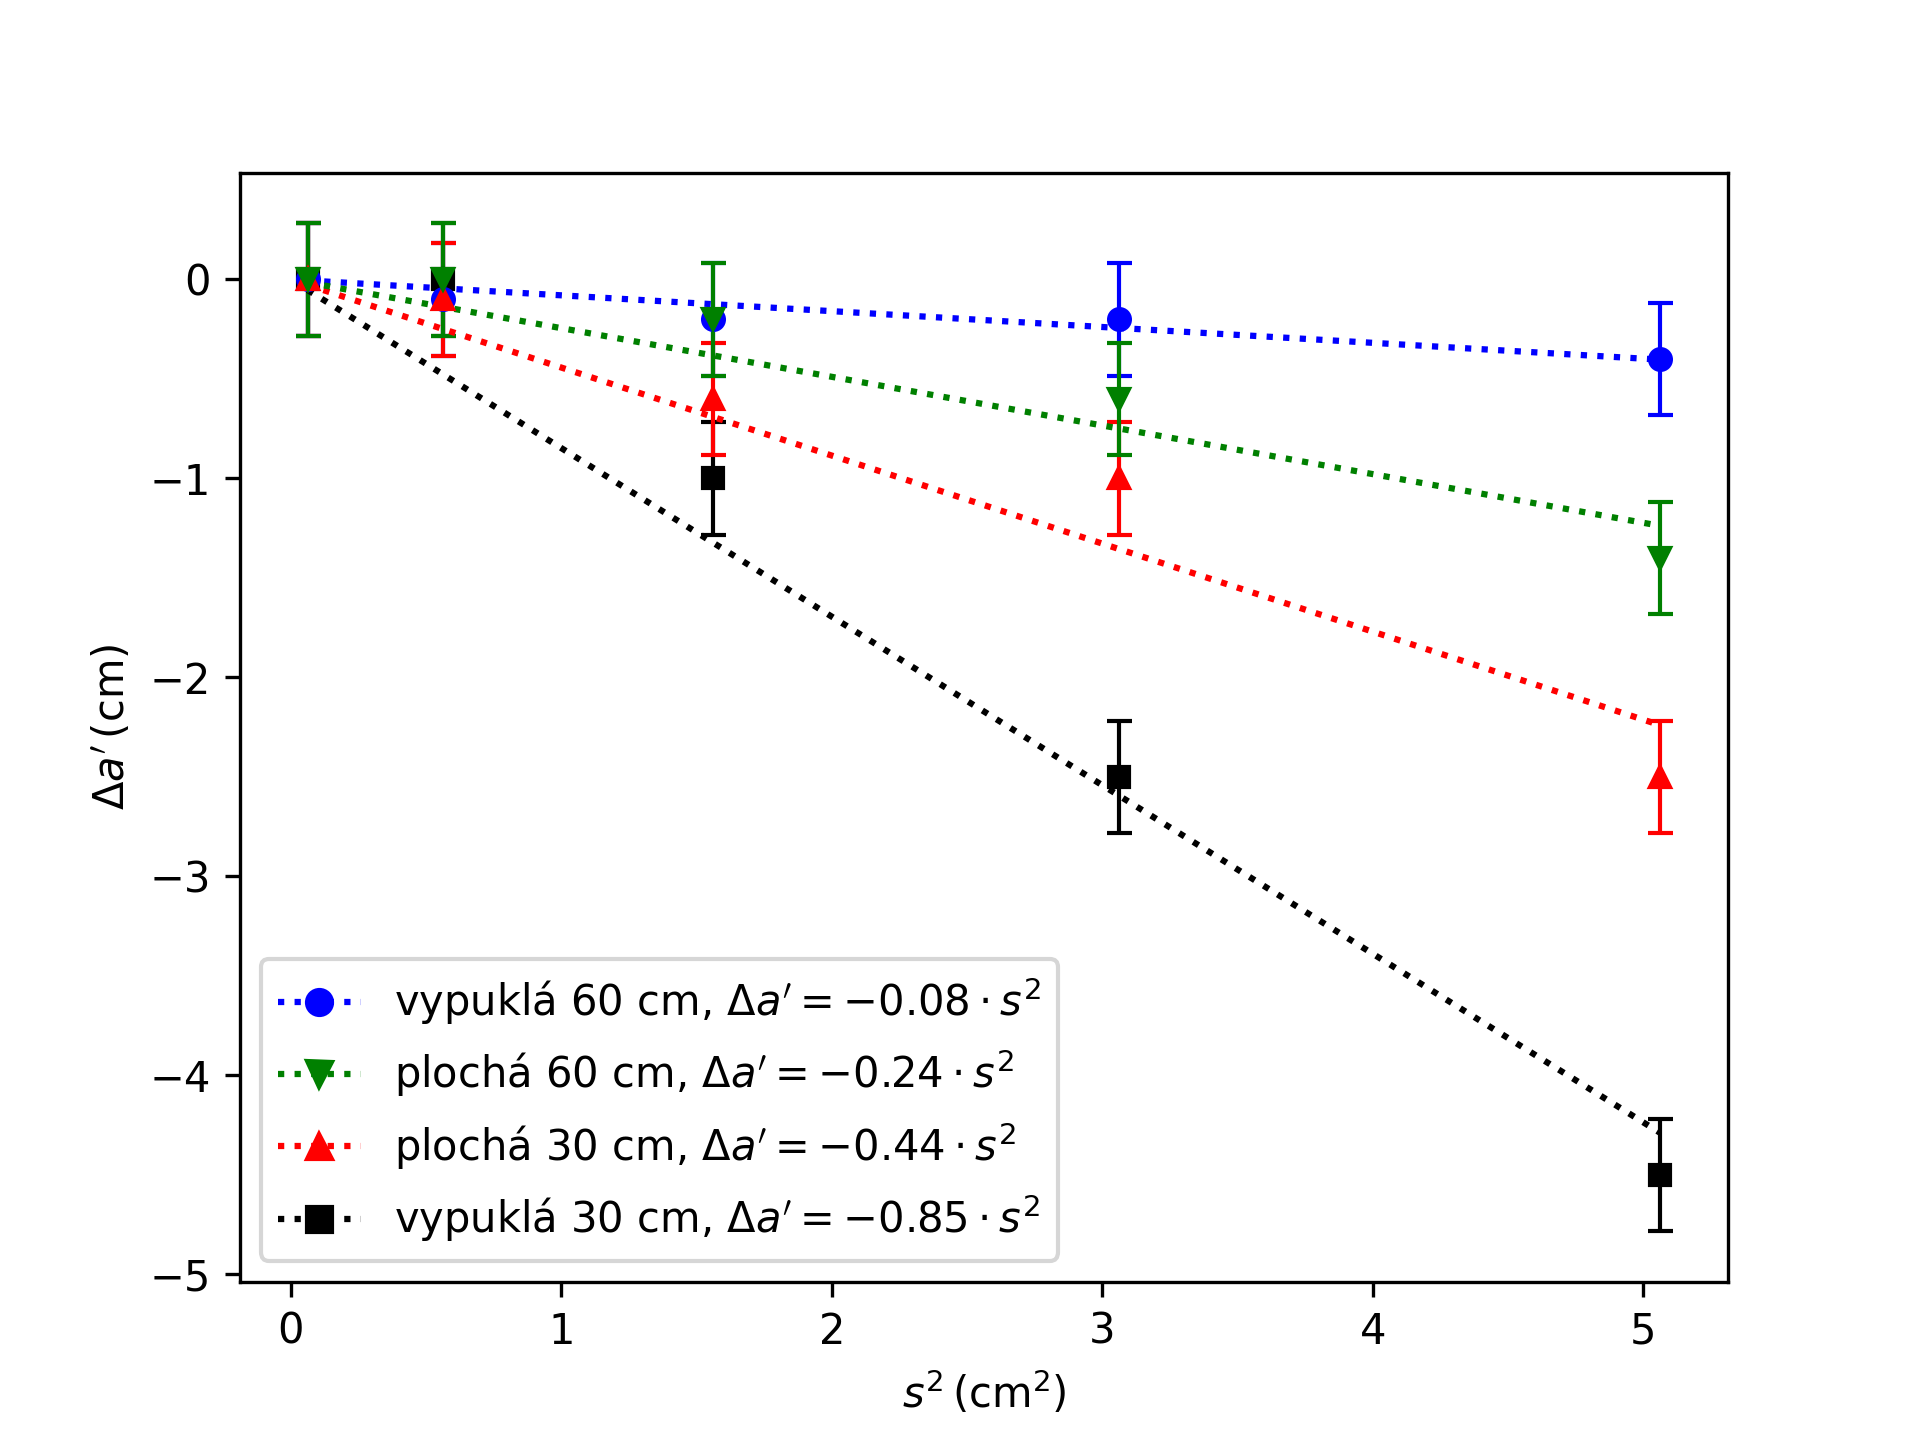
\includegraphics[width=0.5\linewidth]{kulova_vada.png}
    \caption{Závislost kulové vady na kvadrátu vzdálenosti paprsků od optické osy pro~vzdálenost čočky a předmětu $30$ 
    a~$\qty{60}{cm}$ a~pro~oba směry průchodu paprsků čočkou.}
    \label{fig:kulova_vada}
\end{figure}
Datovými body závislosti kulové vady na kvadrátu vzdálenosti paprsků od optické osy byly proloženy přímky procházející počátkem
(ve tvaru $\Delta a' = K s^2$).
Jejich směrnice $K$ byly získány metodou nejmenších čtverců pomocí funkce \texttt{curve\_fit} knihovny \texttt{scipy.optimize}
a~jsou uvedeny v~tabulce \ref{tab:smernice}.

\begin{table}[!htbp]
\centering
\caption{Směrnice závislostí kulové vady na kvadrátu vzdálenosti paprsků od optické osy pro~vzdálenost čočky a předmětu $30$ 
a~$\qty{60}{cm}$ a~pro~oba směry průchodu paprsků čočkou.}
\begin{tabular}{c|c}
 \toprule
 uspořádání & $K\, (\mathrm{cm^{-1}})$ \\
 \midrule
 vypuklá \qty{30}{cm}& $-0.85(5)$ \\
 vypuklá \qty{60}{cm}& $-0.08(5)$ \\
 plochá \qty{30}{cm}& $-0.44(5)$ \\
 plochá \qty{60}{cm}& $-0.24(5)$ \\
 \bottomrule
\end{tabular}
\label{tab:smernice}
\end{table}

% ======================= tloustka a index lomu ----------------- asi hotovo

\subsubsection{Tloušťka čočky, vzdálenost hlavních rovin a index lomu skla.}

Nejistota průměrné hodnoty tloušťky čočky byla určena podle \cite{englich} jako nejistota aritmetického průměru zvětšená
o~nejistotu měřidla:
\begin{equation}
    \label{eq:sigma_mean_t}
    \sigma_{\overline{t}} = \sqrt{ \frac{1}{4 \cdot 5} \sum_{i=1}^{5} \left( t_i - \overline{t} \right)^2
    + \frac{1}{5} \sum_{i=1}^{5} \sigma_{t,B}^2 } \,.
\end{equation}

\begin{table}[!htbp]
\centering
\caption{Změřené tloušťky tenké (čočka 2) a tlusté (čočka 6) čočky.}
\begin{tabular}{c|c|c}
 \toprule
  & tenká & tlustá \\
 \midrule
 číslo měření & $t\, (\mathrm{mm})$ & $t\, (\mathrm{mm})$ \\
 \midrule
 $1$ & $5.77(1)$ & $23.52(1)$ \\
 $2$ & $5.79(1)$ & $23.52(1)$ \\
 $3$ & $5.80(1)$ & $23.55(1)$ \\
 $4$ & $5.78(1)$ & $23.55(1)$ \\
 $5$ & $5.80(1)$ & $23.51(1)$ \\
 \midrule
 průměr & $5.788(7)$ & $23.530(9)$ \\
 \bottomrule
\end{tabular}
\label{tab:tloustky}
\end{table}

% Nejistota pozice hlavní roviny čočky $\sigma_h$ byla kvůli nedostatku času jen odhadnuta na~základě opakovaných měření. 
% Pozice hlavní roviny byla pro~každou čočku změřena několikrát, avšak zaznamenána byla pouze jedna hodnota 
% (jsou uvedeny v~tabulce \ref{tab:hlavni_roviny}).
Kvůli nedostatku času byla zaznamenána pouze jedna hodnota pozice hlavní roviny a~její nejistota byla odhadnuta
na~základě několika opakovaných měření jako $\sigma_h = \qty{0.3}{mm}$.
Nejistota vzdálenosti hlavních rovin byla určena jako:
\begin{equation}
    \label{eq:sigma_delta_h}
    \sigma_\delta = \sqrt{2} \sigma_h \doteq \qty{0.4}{mm} \,.
\end{equation}

\begin{table}[!htbp]
\centering
\caption{Pozice a vzdálenosti hlavních rovin tenké a tlusté čočky určené pomocí goniometru.}
\begin{tabular}{cccc}
 \toprule
 čočka & $h_1 \,(\unit{mm})$ & $h_2 \,(\unit{mm})$ & $\delta \,(\unit{mm})$ \\
 \midrule
 tenká & $19.8(3)$ & $22.0(3)$ & $2.2(4)$  \\
 tlustá & $6.0(3)$ & $16.8(3)$ & $10.8(4)$  \\
 \bottomrule
\end{tabular}
\label{tab:hlavni_roviny}
\end{table}

Index lomu skla tlusté čočky (čočky 6) pro~vlnovou délku $\lambda_\mathrm{Na} = \qty{589.3}{nm}$ byl vypočten podle vztahu 
\ref{eq:index_lomu} jako $n = 1.85(6)$, přičemž jeho 
nejistota byla vypočtena podle \cite{englich} jako:
\begin{equation}
    \label{eq:sigma_n}
    \sigma_n = \frac{1}{\left(t-\delta\right)^2} \sqrt{ \delta^2 \sigma_t^2 + t^2 \sigma_\delta^2} \,.
\end{equation}

Ohnisková vzdálenost tenké čočky (čočka 2) vypočtená Besselovou metodou s~korekcí na~nenulovou vzdálenost hlavních rovin
byla vypočtena podle vztahu \ref{eq:bessel_tlusta} jako $f_{Bessel}' = \qty{20.12(3)}{cm}$, přičemž její nejistota
je daná vztahem \cite{englich}:
\begin{equation}
    \label{eq:sigma_f_bessel_tlusta}
    \sigma_{f_{Bessel}'} = \sqrt{ \left(\frac{\left(D-\delta\right)^2 + \Delta^2}{4 \left(D-\delta\right)^2}\right)^2 
    \left(\sigma_D^2 + \sigma_\delta^2\right) + 
    \left(\frac{\Delta}{2 D}\right)^2 \sigma_{\Delta}^2 } \,.
\end{equation}

\begin{table}[!htbp]
\centering
\caption{Srovnání ohniskových vzdáleností tenké čočky určených různými metodami.}
\begin{tabular}{c|cccc}
 \toprule
 metoda & dvojí zvětšení & Besselova & Besselova s korekcí & z fokometru \\
 \midrule
 $f\,(\unit{cm})$ & $19.9(2)$ & $20.18(3)$ & $20.12(3)$ & $19.0(9)$ \\
 \bottomrule
\end{tabular}
\label{tab:srovnani}
\end{table}

% ============================ DISKUZE a ZÁVĚR ================================
\section{Diskuze výsledků a závěr}
% ======================== diskuze ----------------- asi hotovo
\subsection{Diskuze}
Ohnisková vzdálenost byla metodou dvojího zvětšení určena jako $f_{dvoji} = \qty{19.9(2)}{cm}$ s~relativní nejistotou $1\,\%$,
danou především nejistotou příčných zvětšení (hlavní roli hraje nejistota velikosti předmětu měřená posuvným měřítkem).
Bez korekce na~nenulovou vzdálenost hlavních rovin vychází ohnisková vzdálenost tenké čočky
$f_{Bessel} = \qty{20.18(3)}{cm}$, zatímco s~korekcí $f_{Bessel}' = \qty{20.12(3)}{cm}$, obě hodnoty s~rel. nej. jen $0.15\,\%$
díky tomu, že do nejistoty vstupuje jen nejistota určení pozice čočky, případně obrazu.
Systematická chyba způsobená zanedbáním nenulové
vzdálenosti hlavních rovin má velikost přibližně dvou standardních nejistot, čočku tedy nelze považovat za~tenkou.
Z~optické mohutnosti určené fokometrem vychází ohnisková vzdálenost $f_{fokometr} = \qty{19.0(9)}{cm}$ s~relativní nejistotou $5\,\%$
(danou velikostí nejmenšího dílku stupnice fokometru), jež se~v~rámci nejistoty neshoduje s~ohniskovou vzdáleností
určenou Besselovou metodou. Ze~všech použitých metod je~nejpřesnější Besselova metoda s~korekcí na~vzdálenost hlavních rovin.

V~rámci nejistoty (dané nejistotou určení pozice stínítka, kdy je obraz nejostřejší) je kulová vada skutečně úměrná
kvadrátu vzdálenosti paprsků od~optické osy. Pro~oba směry průchodu paprsků čočkou roste velikost kulové vady se~vzdáleností
paprsků od~osy rychleji ($|K|$ je větší) pro~menší vzdálenost čočky a~předmětu. Pro~vzdálenost \qty{30}{cm} je velikost kulové vady
větší pro~paprsky vstupující do~čočky vypuklou stranou, zatímco pro~vzdálenost \qty{60}{cm} je tomu naopak. Obě závislosti
jsou však relativně podobné, až~do~posledního datového bodu ($s=\qty{2.250(4)}{cm}$) nelze v~rámci nejistoty rozhodnout,
pro~který směr paprsků je kulová vada větší.

Bylo těžké určit přesnou pozici hlavní roviny, tedy polohu, kdy se~při otáčení stolku goniometru nehýbe obraz.
Nejistota byla odhadnuta několikerým změřením jedné pozice hlavní roviny a~byla uvažována stejná pro~obě roviny pro~obě čočky.
Z~toho důvodu vychází relativní nejistota vzdálenosti tlusté čočky $4\,\%$, zatímco tenké čočky až $18\,\%$.

Relativní nejistota indexu lomu tlusté čočky je $3\,\%$, což je dané právě malou přesností určení vzdálenosti hlavních rovin.
Experimentálně určený index lomu odpovídá rozsahu indexů lomu běžných optických skel pro~vlnovou 
délku $\lambda_\mathrm{Na} = \qty{589.3}{nm}$ \cite{edmund}, i když naprostá většina je v~rozmezí $1.5$ až~$1.7$.


% ======================== závěr ----------- asi hotovo
\subsection{Závěr}
Metodou dvojího zvětšení byla určena ohnisková vzdálenost tenké čočky $f_{dvoji} = \qty{19.9(2)}{cm}$. Besselovou metodou
byla získána hodnota $f_{Bessel} = \qty{20.18(3)}{cm}$, přičemž s~korekcí na~nenulovou vzdálenost hlavních rovin vychází hodnota
$f_{Bessel}' = \qty{20.12(3)}{cm}$. Z~optické mohutnosti čočky určené fokometrem byla zjištěna ohnisková vzdálenost 
$f_{fokometr} = \qty{19.0(9)}{cm}$. 

Kulová vada tenké čočky je úměrná kvadrátu vzdálenosti paprsků od optické osy
s~konstantou úměrnosti v~rozmezí $-0.08(5)$ (pro~paprsky vstupující do~čočky vypuklou stranou při~vzdálenosti čočky a~předmětu
\qty{60}{cm}) až~po~$-0.85(5)\,\unit{cm}$ (odpovídající stejnému uspořádání, avšak se~vzdáleností čočky a~předmětu \qty{30}{cm}).
Pro~všechny uspořádán je~konstanta úměrnosti záporná, zkoumaná ploskovypuklá čočka je tedy spojka.

Vzdálenost hlavních rovin tenké čočky byla určena jako $\delta = \qty{2.2(4)}{mm}$ a~tlusté čočky jako 
$\delta = \qty{10.8(4)}{mm}$. Index lomu skla tlusté čočky vychází $n = 1.85(6)$.


% =========================== LITERATURA =============================
\begin{thebibliography}{9}

\bibitem{studijni} Kolektiv ZFP KVOF MFF UK: \textit{Úloha 2 - studijní text} [online]. 
[cit. \today], dostupné z~https://physics.mff.cuni.cz/vyuka/zfp/\_media/zadani/texty/txt\_302.pdf

% \bibitem{pokyny} Kolektiv ZFP KVOF MFF UK: \textit{Úloha 2 - pokyny k měření} [online]. [cit. \today], dostupné
% z~URL

\bibitem{wiki} Wikipedie: Otevřená encyklopedie: \textit{Optická mohutnost} [online]. c2026 [cit. \today], 
dostupné z~https://cs.wikipedia.org/w/index.php?title=Optick\%C3\%A1\_mohutnost\&oldid=25634098

\bibitem{vlnovedelky} Kolektiv ZFP KVOF MFF UK: \textit{Úloha 16 - studijní text} 
[online]. [cit. \today], dostupné
z~https://physics.mff.cuni.cz/vyuka/zfp/\_media/zadani/texty/txt\_316.pdf

\bibitem{englich} J. Englich: \textit{Úvod do praktické fyziky I: Zpracování výsledků měření}. 
1. vyd. Praha: Matfyzpress, 2006


\bibitem{edmund} Edmund Optics Inc.: \textit{Optical Glass - Optical Glass Properties}
[online]. \text{[cit. \today]}, \\
dostupné z~https://www.edmundoptics.com/knowledge-center/application-notes/optics/optical-glass/?srsltid=AfmBOopxB6NqJZ8\_RdpDI8HsBD3Py-egl1W7G153jfHfNS9F-XUjXg9L


% \bibitem{mikulcak} Mikulčák a kolektiv: \textit{Matematické, fyzikální a~chemické tabulky pro~střední 
% školy: NÁZEVTABULKY}, Praha: Státní pedagogické nakladatelství, n. p., 1988

\end{thebibliography}
\end{document}